\section{INTRODUCTION}
\label{sec:intro}

The  most  common  solution  for  the  provision  of  reliable data  storage  is  Redundant Arrays of Independent Disks (RAID) that enables multiple storage elements to be combined to offer a combination of better performance and tolerance to failure.
As RAID systems help achieve a user desired balance between cost, reliability and capacity, they have enjoyed ubiquitous widespread popularity as storage mechanism~\cite{raid_survey}. Several RAID architectures have been proposed. This paper focuses on RAID-6 systems.

While RAID-5 uses only one parity block, RAID-6 extends RAID-5 by adding another parity strip. This allows for two disk failures within the RAID set before any data is lost. The larger the drive capacities and the larger the array size, the more important it becomes to choose RAID 6 instead of RAID-5~\cite{raid6_stop_2019}. Moreover, in current data centers where there are thousands of hard disks, more concurrent disk failures are more frequent, which motivate the need to use systems that tolerate more failures such as RAID-6~\cite{Failure_Trends_2007}.

In this work, we go through a detailed explanation of RAID-6 core design followed by an implementation of this system on top of S3 buckets. Due to the competitive prices on cloud storage, many companies and individuals are using S3 buckets to store their data in different regions~\cite{cloud_2020}. However, some users might want more reliability for their data instead of relaying on a third party implementation. An interesting approach to so is by implementing the RAID-6 system on top of the S3 buckets. We present our detailed analysis of the proposed model and present other possible directions and improvement. 



\begin{figure*}
    \centering
    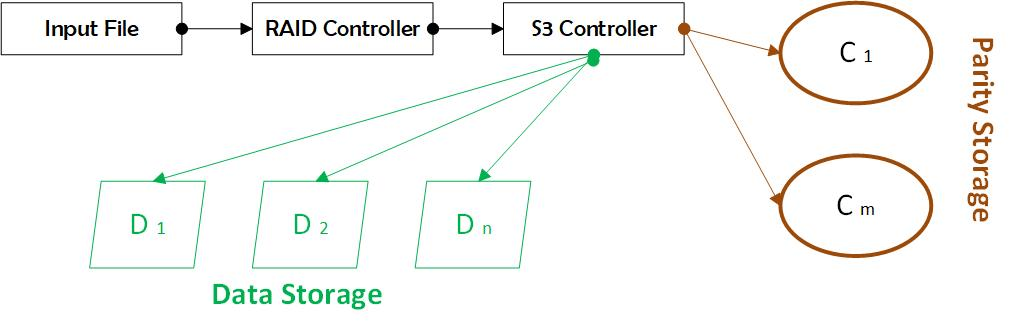
\includegraphics[width=\textwidth]{figures/over_0.jpg}
    \caption {Overview of the S3 based RAID-6 storage architecture}
    \label{fig:overview}
\end{figure*}




The remainder of this paper is organized as follows. In
Section 2, we present our system architecture. Section
3 describes the implementation process. Section 4 and 5 shows
the experiments conducted and the lessons leaned. Finally, in
section 5, we highlight some limitations of RAID-6.




